\flushbottom





%%
%%Plot3D[ Sin[x - t], {x, -4 Pi, 4Pi}, {t, 0, 10} ,
%%       AxesLabel -> {"x", "t", "u"}, Ticks -> None ,
%%       PlotPoints -> 30 ,
%%       ViewPoint -> {0, -2, 1}];
%%




%%============================================================================
%%============================================================================
\chapter{Method of Characteristics}










%%============================================================================
\section{First Order Linear Equations}




Consider the following first order wave equation.
\begin{equation}
  \label{eqn ut+cux=0}
  u_t + c u_x = 0
\end{equation}
Let $x(t)$ be some path in the phase plane.  Perhaps $x(t)$ describes the
position of an observer who is noting the value of the solution $u(x(t),t)$
at their current location.  We differentiate with respect to $t$ to see 
how the solution varies for the observer.
\begin{equation}
  \label{eqn ddtuxt=ut+xux}
  \frac{\dd}{\dd t} u(x(t),t) = u_t + x'(t) u_x
\end{equation}
We note that if the observer is moving with velocity $c$, $x'(t) = c$, 
then the solution at their current location does not change because
$u_t + c u_x = 0$.  We will examine this more carefully.

By comparing Equations~\ref{eqn ut+cux=0} and~\ref{eqn ddtuxt=ut+xux} we 
obtain ordinary differential equations representing the position of an 
observer and the value of the solution at that position.
\[
\frac{\dd x}{\dd t} = c, \quad \frac{\dd u}{\dd t} = 0
\]
Let the observer start at the position $x_0$.  Then we have an initial value
problem for $x(t)$.
\begin{gather*}
  \frac{\dd x}{\dd t} = c, \quad x(0) = x_0
  \\
  x(t) = x_0 + c t
\end{gather*}
These lines $x(t)$ are called \textit{characteristics} of 
Equation~\ref{eqn ut+cux=0}.

Let the initial condition be $u(x,0) = f(x)$.  We have an initial value 
problem for $u(x(t),t)$.
\begin{gather*}
  \frac{\dd u}{\dd t} = 0, \quad u(0) = f(x_0)
  \\
  u(x(t),t) = f(x_0)
\end{gather*}
Again we see that the solution is constant along the characteristics.
We substitute the equation for the characteristics into this expression.
\begin{gather*}
  u(x_0 + c t,t) = f(x_0)
  \\
  u(x,t) = f(x - c t)
\end{gather*}
Now we see that the solution of Equation~\ref{eqn ut+cux=0} is a wave moving
with velocity $c$.  The solution at time $t$ is the initial condition 
translated a distance of $c t$.







%%============================================================================
\section{First Order Quasi-Linear Equations}




Consider the following quasi-linear equation.
\begin{equation}
  \label{eqn ut+axtuux=0}
  u_t + a(x,t,u) u_x = 0
\end{equation}
We will solve this equation with the method of characteristics.
We differentiate the solution along a path $x(t)$.
\begin{equation}
  \label{eqn ddtuxt=ut+xux 2}
  \frac{\dd}{\dd t} u(x(t),t) = u_t + x'(t) u_x
\end{equation}
By comparing Equations~\ref{eqn ut+axtuux=0} and~\ref{eqn ddtuxt=ut+xux 2} we 
obtain ordinary differential equations for the characteristics $x(t)$ and
the solution along the characteristics $u(x(t),t)$.
\[
\frac{\dd x}{\dd t} = a(x,t,u), \quad \frac{\dd u}{\dd t} = 0
\]
Suppose an initial condition is specified, $u(x,0) = f(x)$.  Then we have 
ordinary differential equation, initial value problems.
\begin{gather*}
  \frac{\dd x}{\dd t} = a(x,t,u), \quad x(0) = x_0
  \\
  \frac{\dd u}{\dd t} = 0, \quad u(0) = f(x_0)
\end{gather*}
We see that the solution is constant along the characteristics.
The solution of Equation~\ref{eqn ut+axtuux=0} is a wave moving
with velocity $a(x,t,u)$.





\begin{Example}
  Consider the inviscid Burger equation,
  \[
  u_t + u u_x = 0, \quad u(x,0) = f(x).
  \]
  We write down the differential equations for the solution along a 
  characteristic.
  \begin{gather*}
    \frac{\dd x}{\dd t} = u, \quad x(0) = x_0
    \\
    \frac{\dd u}{\dd t} = 0, \quad u(0) = f(x_0)
  \end{gather*}
  First we solve the equation for $u$.  $u = f(x_0)$.  Then we solve for $x$.
  $x = x_0 + f(x_0) t$.  This gives us an implicit solution of the Burger equation.
  \[
  u(x_0 + f(x_0) t, t) = f(x_0)
  \]
  %% CONTINUE
\end{Example}






%%The method of characteristics is used to solve first order 
%%quasi-linear partial differential equations.  Consider the partial 
%%differential equation
%%\[ a u_x + b u_y = u, \quad u(0,y) = f(y).\]
%%The derivative of $u$ with respect to some variable, $s$, is
%%\[ \frac{\dd u}{\dd s} = \left(\frac{\partial x}{\partial s}\right) u_x +
%%                \left(\frac{\partial y}{\partial s}\right)u_y.\]
%%Comparing the above two equations we see that the partial differential equation is equivalent to the
%%system of ODE's
%%\begin{alignat*}{3}
%%&\frac{\partial x}{\partial s} = a     &\qquad &\frac{\partial y}{\partial s} = b     &\qquad
%%        &\frac{\dd u}{\dd s} = u \\
%%\intertext{The initial condition corresponds to}
%%&x(s=0) = 0             &\qquad &y(s=0) = \alpha        &\qquad
%%        &u(s=0) = f(\alpha) \\
%%\intertext{Here, $s$ and $\alpha$ are the new independent variables.
%%Solving these ODE's yields}
%%&x=as                   &\qquad &y=b s+\alpha            &\qquad
%%        &u=\e^s f(\alpha).\\
%%\intertext{We can solve for $s$ and $\alpha$ and substitute these
%%variables into the expression for $u$.}
%%&s= x/a                 &\qquad &\alpha = y-b x/a        &\qquad
%%        &u = \e^{x/a}f(y-b x/a)
%%\end{alignat*}
%%Thus the solution to the partial differential equation is
%%\[ \boxed{u(x,y) = \e^{x/a}f(y-b x/a)}.\]




%%\vspace{.2in}
%%As another example of the method, consider the following problem from
%%``Handbook of Differential Equations'' by Zwillinger.
%%\[u_x + x^2 u_y = - y u,\quad u(0,y) = f(y).\]
%%The corresponding system of ODE's and initial conditions are
%%\begin{alignat*}{3}
%%&\frac{\partial x}{\partial s} = 1     &\qquad &\frac{\partial y}{\partial s} = x^2   &\qquad
%%        &\frac{\dd u}{\dd s} = -y u \\
%%&x(s=0) = 0             &\qquad &y(s=0) = \alpha        &\qquad
%%        &u(s=0) = f(\alpha) \\
%%\intertext{Solving the ODE's and substituting in the values of the variables
%%yields}
%%&x = s                  &\qquad &\frac{\partial y}{\partial s} = s^2   &       & \\
%%&x = s                  &\qquad &y = \frac{s^3}{3}+\alpha       &\qquad
%%        &\frac{\dd u}{\dd s} = - (\frac{s^3}{3}+\alpha)u  \\
%%&s = x                  &\qquad &\alpha=y - \frac{x^3}{3}       &\qquad
%%        &u = f(\alpha)\exp\left(-\frac{s^4}{12}-s\alpha\right)  \\
%%\end{alignat*}
%%Thus the solution is
%%\[ \boxed{u(x,y) = f\left(y- \frac{x^3}{3}\right)
%%        \exp\left(\frac{x^4}{4}-x y \right).} \]














%%=============================================================================
\section{The Method of Characteristics and the Wave Equation}



Consider the one dimensional wave equation,
\[
u_{t t} = c^2 u_{x x}.
\]
We make the change of variables, $a = u_x$, $b = u_t$, to obtain a coupled 
system of first order equations.
\begin{align*}
  a_t - b_x &= 0 \\
  b_t - c^2 a_x &= 0
\end{align*}
We write this as a matrix equation.
\[
\begin{pmatrix} a \\ b \end{pmatrix}_t + 
\begin{pmatrix} 0 & -1 \\ -c^2 & 0 \end{pmatrix}
\begin{pmatrix} a \\ b \end{pmatrix}_x = 0
\]
The eigenvalues and eigenvectors of the matrix are 
\[
\lambda_1 = -c, \quad \lambda_2 = c, \qquad 
\boldsymbol{\xi}_1 = \begin{pmatrix} 1 \\ c \end{pmatrix}, \quad 
\boldsymbol{\xi}_2 = \begin{pmatrix} 1 \\ -c \end{pmatrix}.
\]
The matrix is diagonalized by a similarity transformation.
\[
\begin{pmatrix} -c & 0 \\ 0 & c \end{pmatrix}
=
\begin{pmatrix} 1 & 1 \\ c & -c \end{pmatrix}^{-1} 
\begin{pmatrix} 0 & -1 \\ -c^2 & 0 \end{pmatrix}
\begin{pmatrix} 1 & 1 \\ c & -c \end{pmatrix}
\]
We make a change of variables to diagonalize the system.
\begin{gather*}
  \begin{pmatrix} a \\ b \end{pmatrix}
  =
  \begin{pmatrix} 1 & 1 \\ c & -c \end{pmatrix}
  \begin{pmatrix} \alpha \\ \beta \end{pmatrix}
  \\
  \begin{pmatrix} 1 & 1 \\ c & -c \end{pmatrix}
  \begin{pmatrix} \alpha \\ \beta \end{pmatrix}_t + 
  \begin{pmatrix} 0 & -1 \\ -c^2 & 0 \end{pmatrix}
  \begin{pmatrix} 1 & 1 \\ c & -c \end{pmatrix}
  \begin{pmatrix} \alpha \\ \beta \end{pmatrix}_x = 0
\end{gather*}
Now we left multiply by the inverse of the matrix of eigenvectors to obtain
an uncoupled system that we can solve directly.
\begin{gather*}
  \begin{pmatrix} \alpha \\ \beta  \end{pmatrix}_t + 
  \begin{pmatrix} -c & 0 \\ 0 & c \end{pmatrix}
  \begin{pmatrix} \alpha \\ \beta \end{pmatrix}_x = 0.
  \\
  \alpha(x,t) = p(x + c t), \quad \beta(x,t) = q(x - c t),
\end{gather*}
Here $p,q \in C^2$ are arbitrary functions.
We change variables back to $a$ and $b$.
\[
a(x,t) = p(x + c t) + q(x - c t), \qquad
b(x,t) = c p(x + c t) - c q(x - c t)
\]
We could integrate either $a = u_x$ or  $b = u_t$ to obtain the solution of 
the wave equation.
\[
\boxed{
  u = F(x - c t) + G(x + c t)
  }
\]
Here $F,G \in C^2$ are arbitrary functions.  
We see that $u(x,t)$ is the sum of a waves moving to the right and left
with speed $c$.  This is the general solution 
of the one-dimensional wave equation.  Note that for any given
problem, $F$ and $G$ are only determined to whithin an additive
constant.  For any constant $k$, adding $k$ to $F$ and subtracting
it from $G$ does not change the solution.
\[
u = \left( F(x - c t) + k \right) + \left( G(x - c t) - k \right)
\]









%%==============================================================================
%%\section{The Method of Characteristics and the Wave Equation}
%%Consider the one dimensional wave equation
%%\[ u_{t t} -c^2 u_{x x} = 0.\]
%%We can factor this equation into
%%\[ \left(\frac{\partial}{\partial t} + c\frac{\partial}{\partial x}\right)
%%        \left(\frac{\partial u}{\partial t} - c\frac{\partial u}{\partial x}\right) = 0.\]
%%Thus we can rewrite the wave equation as a system of first order PDE's
%%\begin{align*}
%%&w_t + c w_x = 0 \\
%%&u_t - c u_x = w.
%%\end{align*}
%%We can now apply the method of characteristics.  Assume that the initial
%%conditions for the system are
%%\[ u(x,0) = f(x),\qquad w(x,0) = g(x).\]
%%Differentiating $w$ with respect to $s$ yields
%%\[\frac{\dd w}{\dd s} = \left(\frac{\partial t}{\partial s}\right)w_t
%%        + \left(\frac{\partial x}{\partial s}\right)w_x.\]
%%Thus the PDE for $w$ and its initial condition yield
%%\begin{alignat*}{3}
%%&\frac{\partial t}{\partial s} = 1     &\qquad &\frac{\partial x}{\partial s} = c             &\qquad
%%        &\frac{\dd w}{\dd s} = 0 \\
%%&t(s=0,\alpha)= 0       &\qquad &x(s=0,\alpha)= \alpha          &\qquad
%%        &w(s=0,\alpha) = g(\alpha).\\
%%\intertext{Solving these equations,}
%%&t=s                    &\qquad &x = c s + \alpha                &\qquad
%%        &w = g(\alpha) \\
%%&s=t                    &\qquad &\alpha = x -c t                 &\qquad
%%        &w = g(x-c t).
%%\end{alignat*}
%%
%%Thus we see that $w$ is a function of $x-c t$.  Now we solve the first
%%order equation for $u$ with the method of characteristics.
%%
%%\begin{alignat*}{3}
%%&\frac{\partial t}{\partial s} = 1     &\qquad &\frac{\partial x}{\partial s} = -c            &\qquad
%%        &\frac{\dd u}{\dd s} = w=g(x-c t) \\
%%&t(s=0,\alpha)= 0       &\qquad &x(s=0,\alpha)= \alpha          &\qquad
%%        &w(s=0,\alpha) = f(\alpha).\\
%%\intertext{Solving these equations,}
%%&t=s                    &\qquad &x = -c s + \alpha               &\qquad
%%        &\frac{\dd u}{\dd s} = g(-c s+\alpha -c s) \\
%%&s=t                    &\qquad &\alpha = x +c t                 &\qquad
%%        &u = \int g(\alpha-2c s)d s + f(\alpha) \\
%%&s=t                    &\qquad &\alpha = x +c t                 &\qquad
%%        &u = h(\alpha-2c s) + f(\alpha) \\
%%&s=t                    &\qquad &\alpha = x +c t                 &\qquad
%%        &u = h(x-c t) + f(x+c t).
%%\end{alignat*}
%%Thus the solution to the wave equation is
%%\[\boxed{u(x,t) = F(x+c t) + G(x-c t)}\]
%%where $F$ and $G$ are functions that depend on the initial conditions.
%%
%%
%%
%%






%%==============================================================================
\section{The Wave Equation for an Infinite Domain}




Consider the Cauchy problem for the wave equation on $-\infty < x < \infty$.
\begin{gather*}
  u_{t t} = c^2 u_{x x}, \quad -\infty < x < \infty, \ t > 0 \\
  u(x,0) = f(x), \qquad u_t(x,0) = g(x)
\end{gather*}
We know that the solution is the sum of right-moving and left-moving waves.
\begin{equation}
  \label{u(xt)=f(x+ct)+g(x-ct)}
  u(x,t) = F(x - c t) + G(x + c t)
\end{equation}
The initial conditions give us two constraints on $F$ and $G$.
\[
F(x) + G(x) = f(x), \quad
- c F'(x) + c G'(x) = g(x).
\]
We integrate the second equation.
\[
- F(x) + G(x) = \frac{1}{c} \int g(x)\,\dd x + \mathrm{const}
\]
Here $Q(x) = \int q(x) \,\dd x$.
We solve the system of equations for $F$ and $G$.
\[
F(x) = \frac{1}{2} f(x) - \frac{1}{2c} \int g(x)\,\dd x - k, \quad
G(x) = \frac{1}{2} f(x) + \frac{1}{2c} \int g(x)\,\dd x + k
\]
Note that the value of the constant $k$ does not affect the solution, $u(x,t)$.
For simplicity we take $k = 0$.  We substitute $F$ and $G$ into 
Equation~\ref{u(xt)=f(x+ct)+g(x-ct)} to determine the solution.
\begin{gather*}
  u(x,t) = \frac{1}{2} \left( f(x - c t) + f(x + c t) \right)
  + \frac{1}{2c} \left( \int^{x + c t} g(x)\,\dd x - \int^{x - c t} g(x)\,\dd x \right) 
  \\
  u(x,t) = \frac{1}{2} \left( f(x - c t) + f(x + c t) \right)
  + \frac{1}{2c} \int_{x - c t}^{x + c t} g(\xi) \,\dd \xi \\
  \boxed{
    u(x,t) = \frac{1}{2} \left( u(x - c t,0) + u(x + c t,0) \right)
    + \frac{1}{2c} \int_{x - c t}^{x + c t} u_t(\xi,0) \,\dd \xi
    }
\end{gather*}








%%==============================================================================
\section{The Wave Equation for a Semi-Infinite Domain}





Consider the wave equation for a semi-infinite domain.
\begin{gather*}
  u_{t t} = c^2 u_{x x}, \quad 0 <  x < \infty, \ t > 0 \\
  u(x,0) = f(x), \qquad u_t(x,0) = g(x), \qquad u(0,t) = h(t)
\end{gather*}
Again the solution is the sum of a right-moving and a left-moving wave.
\[
u(x,t) = F(x - c t) + G(x + c t)
\]
For $x > c t$, the boundary condition at $x = 0$ does not affect the solution.
Thus we know the solution in this domain from our work on the wave equation
in the infinite domain.
\[
u(x,t) = \frac{1}{2} \left( f(x - c t) + f(x + c t) \right)
+ \frac{1}{2c} \int_{x - c t}^{x + c t} g(\xi) \,\dd \xi, \quad x > c t
\]
From this, $F(\xi)$ and $G(\xi)$ are determined for $\xi > 0$.
\begin{gather*}
  F(\xi) = \frac{1}{2} f(\xi) - \frac{1}{2c} \int g(\xi) \,\dd \xi, \quad \xi > 0
  \\
  G(\xi) = \frac{1}{2} f(\xi) + \frac{1}{2c} \int g(\xi) \,\dd \xi, \quad \xi > 0
\end{gather*}

In order to determine the solution $u(x,t)$ for $x,t > 0$ we also need to 
determine $F(\xi)$ for $\xi < 0$.  To do this, we substitute the form of the 
solution into the boundary condition at $x = 0$.
\begin{gather*}
  u(0,t) = h(t), \quad t > 0
  \\
  F(-c t) + G(c t) = h(t), \quad  t > 0 
  \\
  F(\xi) = -  G(-\xi) + h(-\xi/c), \quad \xi < 0 
  \\
  F(\xi) = - \frac{1}{2} f(-\xi) - \frac{1}{2c} \int^{-\xi} g(\psi) \,\dd \psi + h(-\xi/c), 
  \quad \xi < 0
\end{gather*}
We determine the solution of the wave equation for $x < c t$.
\begin{gather*}
  u(x,t) = F(x - c t) + G(x + c t)
  \\
  u(x,t) = - \frac{1}{2} f(-x + c t) - \frac{1}{2c} \int^{-x + c t} g(\xi) \,\dd \xi 
  + h(t - x/c)
  + \frac{1}{2} f(x + c t) + \frac{1}{2c} \int^{x + c t} g(\xi) \,\dd \xi, \quad x < c t
  \\
  u(x,t) = \frac{1}{2} \left( - f(-x + c t) + f(x + c t) \right)
  + \frac{1}{2c} \int_{-x + c t}^{x + c t} g(\xi) \,\dd \xi + h(t - x/c), \quad x < c t
\end{gather*}
Finally, we collect the solutions in the two domains.
\[
\boxed{
  u(x,t) = \begin{cases}
    \frac{1}{2} \left( f(x - c t) + f(x + c t) \right)
    + \frac{1}{2c} \int_{x - c t}^{x + c t} g(\xi) \,\dd \xi, &x > c t
    \\
    \frac{1}{2} \left( - f(-x + c t) + f(x + c t) \right)
    + \frac{1}{2c} \int_{-x + c t}^{x + c t} g(\xi) \,\dd \xi + h(t - x/c), &x < c t
  \end{cases}
  }
\]









%%==============================================================================
\section{The Wave Equation for a Finite Domain}


%% CONTINUE: Do inhomogeneous boundary conditions.


Consider the wave equation for the infinite domain.
\begin{gather*}
  u_{t t} = c^2 u_{x x}, \quad -\infty <  x < \infty, \ t > 0 
  \\
  u(x,0) = f(x), \qquad u_t(x,0) = g(x)
\end{gather*}
If $f(x)$ and $g(x)$ are odd about $x = 0$, ($f(x) = - f(-x)$,
$g(x) = - g(-x)$), then $u(x,t)$ is also odd about $x = 0$.  We can 
demonstrate this with D'Alembert's solution.
\[
u(x,t) = \frac{1}{2} \left( f(x - c t) + f(x + c t) \right)
+ \frac{1}{2c} \int_{x - c t}^{x + c t} g(\xi) \,\dd \xi
\]
\begin{align*}
  - u(-x,t)
  &= - \frac{1}{2} \left( f(- x - c t) + f(- x + c t) \right)
  - \frac{1}{2c} \int_{-x - c t}^{-x + c t} g(\xi) \,\dd \xi
  \\
  &= \frac{1}{2} \left( f(x + c t) + f(x - c t) \right)
  - \frac{1}{2c} \int_{x + c t}^{x - c t} g(-\xi) \,(-\dd \xi)
  \\
  &= \frac{1}{2} \left( f(x - c t) + f(x + c t) \right)
  + \frac{1}{2c} \int_{x - c t}^{x + c t} g(\xi) \,\dd \xi
  \\
  &= u(x,t)
\end{align*}
Thus if the initial conditions $f(x)$ and $g(x)$ are odd about a 
point then the solution of the wave equation $u(x,t)$ is also odd about 
that point.  The analogous result holds if the initial conditions are even
about a point.  These results are useful in solving the wave equation on
a finite domain.





Consider a string of length $L$ with fixed ends.
\begin{gather*}
  u_{t t} = c^2 u_{x x}, \quad 0 < x < L, \ t > 0 
  \\
  u(x,0) = f(x), \quad u_t(x,0) = g(x), \quad
  u(0,t) = u(L,t) = 0
\end{gather*}
We extend the domain of the problem to $x \in (-\infty \ldots \infty)$.  We form the odd
periodic extensions $\tilde{f}$ and $\tilde{g}$ which are odd about the 
points $x = 0,L$.  

If a function $h(x)$ is defined for positive $x$, then $\sign(x) h(|x|)$ is 
the odd extension of the function.  If $h(x)$ is defined for $x \in (-L \ldots L)$ 
then its periodic extension is 
\[
h \left( x - 2 L \left\lfloor \frac{x+L}{2L} \right\rfloor \right).
\]
We combine these two formulas to form odd periodic extensions.
\begin{gather*}
  \tilde{f}(x) = 
  \sign \left( x - 2 L \left\lfloor \frac{x+L}{2L} \right\rfloor \right)
  f \left( \left| x - 2 L \left\lfloor \frac{x+L}{2L} \right\rfloor \right| \right)
  \\
  \tilde{g}(x) = 
  \sign \left( x - 2 L \left\lfloor \frac{x+L}{2L} \right\rfloor \right)
  g \left( \left| x - 2 L \left\lfloor \frac{x+L}{2L} \right\rfloor \right| \right)
\end{gather*}
Now we can write the solution for the vibrations of a string with fixed ends.
\[
u(x,t) = \frac{1}{2} \left( \tilde{f}(x - c t) + \tilde{f}(x + c t) \right)
+ \frac{1}{2c} \int_{x - c t}^{x + c t} \tilde{g}(\xi) \,\dd \xi
\]








%%=============================================================================
\section{Envelopes of Curves}






Consider the tangent lines to the parabola $y=x^2$.  The slope of the tangent
at the point $(x,x^2)$ is $2x$.  The set of tangents form a one
parameter family of lines,
\[
f(x,t) = t^2 + (x-t)2t = 2 t x - t^2.
\]
The parabola and some of its tangents are plotted in Figure~\ref{partan}.

%%In[1]:=
%%\!\(\(parTan[x_, t_] := {x + t, x\^2 + 2  x\ t}; \)\)
%%In[2]:=
%%\!\(\(Plot[x\^2, {x, \(-1\), 1}, AspectRatio -> Automatic]; \)\)
%%In[3]:=
%%ParametricPlot[Evaluate[Table[parTan[x,t],{x,-1,1,1/5}]],{t,-2,2},
%%  AspectRatio->Automatic];
%%In[4]:=
%%Show[%%,%%%%,PlotRange->{{-1,1},{-1,1}},AspectRatio->Automatic,
%%  Ticks->{{-1,0,1},{-1,0,1}}];

\begin{figure}[h!]
  \begin{center}
    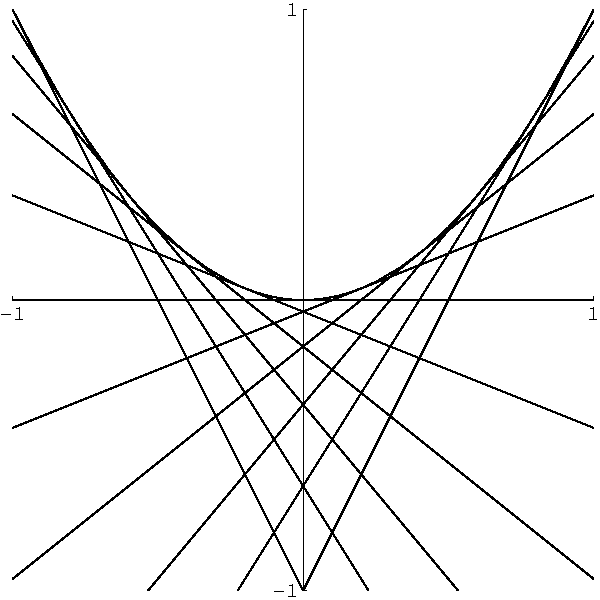
\includegraphics[width=0.4\textwidth]{pde/characteristics/partan}
  \end{center}
  \caption{A parabola and its tangents.}
  \label{partan}
\end{figure}

%% CONTINUE: Give a satisfactory definition of envelope.

The parabola is the \textit{envelope} of the family of tangent lines.  
Each point on the parabola is tangent to one of the lines.
Given a curve, we can generate a family of lines that envelope the curve.
We can also do the opposite, given a family of lines, we can determine the
curve that they envelope.  More generally, given a family of curves, 
we can determine the curve that they envelope.  Let the one parameter
family of curves be given by the equation $F(x,y,t) = 0$.  For the 
example of the tangents to the parabola this equation would be
$y - 2 t x + t^2 = 0$.


%% CONTINUE: The explanation here really sucks.
Let $y(x)$ be the envelope of $F(x,y,t)=0$.  Then the points on $y(x)$ 
must lie on the family of curves.  Thus $y(x)$ must satisfy the 
equation $F(x,y,t)=0$.  The points that lie on the envelope have the 
property,
\[
\frac{\partial}{\partial t} F(x,y,t) = 0.
\]
We can solve this equation for $t$ in terms of $x$ and $y$, $t=t(x,y)$.
The equation for the envelope is then
\[
F(x,y,t(x,y)) = 0.
\]

Consider the example of the tangents to the parabola.  The equation of
the one-parameter family of curves is
\[
F(x,y,t) \equiv y - 2 t x + t^2 = 0.
\]
The condition $F_t(x,y,t)=0$ gives us the constraint,
\[
-2 x + 2 t = 0.
\]
Solving this for $t$ gives us $t(x,y) = x$.  The equation for the 
envelope is then,
\[
y - 2 x x + x^2 = 0,
\]
\[
y = x^2.
\]




\begin{Example}
  Consider the one parameter family of curves,
  \[
  (x-t)^2 + (y-t)^2 - 1 = 0.
  \]
  These are circles of unit radius and center $(t,t)$.  To determine the 
  envelope of the family, we first use the constraint $F_t(x,y,t)$ to 
  solve for $t(x,y)$.
  \[
  F_t(x,y,t) = -2(x-t) - 2(y-t) = 0
  \]
  \[
  t(x,y) = \frac{x+y}{2}
  \]
  Now we substitute this into the equation $F(x,y,t)=0$ to determine the 
  envelope.
  \[
  F \left( x,y,\frac{x+y}{2} \right) 
  = \left(x - \frac{x+y}{2} \right)^2 + \left(y - \frac{x+y}{2} \right)^2 - 1 = 0
  \]
  \[
  \left(\frac{x-y}{2} \right)^2 + \left(\frac{y-x}{2} \right)^2 - 1 = 0
  \]
  \[
  (x-y)^2 = 2
  \]
  \[
  \boxed{
    y = x \pm \sqrt{2}
    }
  \]
  The one parameter family of curves and its envelope is shown in 
  Figure~\ref{circlefamily}.

  %%In[5]:=
  %%cf[\[Theta]_,t_]:={t+Cos[\[Theta]],t+Sin[\[Theta]]};
  %%In[8]:=
  %%ParametricPlot[
  %%  Evaluate[Table[cf[\[Theta],t],{t,-2,2,1/3}]],{\[Theta],0,2\[Pi]}];
  %%In[9]:=
  %%\!\(\(Plot[{x - \@2, x + \@2}, {x, \(-3\), 3}]; \)\)
  %%In[10]:=
  %%Show[%%,%%%%,PlotRange->{{-3,3},{-3,3}},AspectRatio->Automatic];



  \begin{figure}[h!]
    \begin{center}
      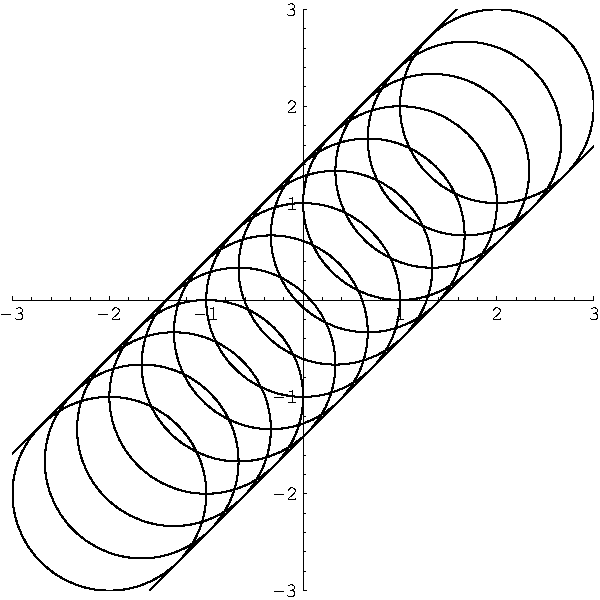
\includegraphics[width=0.4\textwidth]{pde/characteristics/circle}
    \end{center}
    \caption{The one parameter family of curves and its envelope.}
    \label{circlefamily}
  \end{figure}
\end{Example}






































\raggedbottom
%%=============================================================================
\exercises{
\pagebreak
\flushbottom
\section{Exercises}








\begin{Exercise}
  Consider the small transverse vibrations of a composite string of
  infinite extent, made up of two homogeneous strings of different densities 
  joined at $x = 0$. In each region 1) $x < 0$, 2) $x > 0$ we have
  \[
  u_{t t} - c_j^2 u_{x x} = 0 \quad j = 1,2  \quad c_1 \neq c_2,
  \]
  and we require continuity of $u$ and $u_x$ at $x = 0$. Suppose for $t < 0$ a 
  wave approaches the junction $x = 0$ from the left, i.e. as $t$ approaches 
  $0$ from negative values:
  \[ 
  u(x,t) = \begin{cases}
    F(x-c_1t) & x < 0, t \leq 0 \\
    0 &x > 0, t \leq 0 
  \end{cases}
  \] 
  As $t$ increases further, the wave reaches $x = 0$ and gives rise to reflected
  and transmitted waves.

  \begin{enumerate} 
  \item 
    Formulate the appropriate initial values for $u$ at $t = 0$. 
  \item 
    Solve the initial-value problem for $-\infty < x < \infty$ , $t > 0$. 
  \item 
    Identify the incident, reflected and transmitted waves in your solution 
    and determine the reflection and transmission coefficients for the junction
    in terms of $c_1$ and $c_2$. Comment also on their values in the limit
    $c_1 \to c_2$. 
  \end{enumerate} 
\end{Exercise}












%% 1D wave equation, 0 < x < \infty, -\infty < t < \infty.
\begin{Exercise}
  Consider a semi-infinite string, $x > 0$.  For all time the end of the
  string is displaced according to $u(0, t) = f(t)$.  Find the motion of 
  the string, $u(x, t)$ with the method of characteristics
  and then with a Fourier transform in time.  The wave speed is $c$.
\end{Exercise}




%%u u_x + u_y = 1, \quad u \big|_{x=y} = \frac{x}{2}.
\begin{Exercise}
  Solve using characteristics:
  \[
  u u_x + u_y = 1, \quad u \big|_{x=y} = \frac{x}{2}.
  \]
\end{Exercise}




%%(y + u) u_x + y u_y = x - y, \quad u \big|_{y=1} = 1 + x.
\begin{Exercise}
  Solve using characteristics:
  \[
  (y + u) u_x + y u_y = x - y, \quad u \big|_{y=1} = 1 + x.
  \]
\end{Exercise}






\raggedbottom
}
%%=============================================================================
\hints{
\pagebreak
\flushbottom
\section{Hints}






\begin{Hint}
  %% CONTINUE
\end{Hint}






%% 1D wave equation, 0 < x < \infty, -\infty < t < \infty.
\begin{Hint}
  \begin{enumerate}
  \item
    Because the left end of the string is being displaced, there will only 
    be right-moving waves.  Assume a solution of the form
    \[
    u(x,t) = F(x - c t).
    \]
  \item
    Take a Fourier transform in time.  Use that there are only outgoing waves.
  \end{enumerate}
\end{Hint}





%%u u_x + u_y = 1, \quad u \big|_{x=y} = \frac{x}{2}.
\begin{Hint}
  %% CONTINUE
\end{Hint}



%%(y + u) u_x + y u_y = x - y, \quad u \big|_{y=1} = 1 + x.
\begin{Hint}
  %% CONTINUE
\end{Hint}
















\raggedbottom
}
%%=============================================================================
\solutions{
\pagebreak
\flushbottom
\section{Solutions}








\begin{Solution}
  \begin{enumerate} 
  \item 
    \begin{gather*}
      u(x,0) = \begin{cases}
        F(x), &x < 0 \\
        0, &x > 0
      \end{cases}
      \\
      u_t(x,0) = \begin{cases}
        - c_1 F'(x), &x < 0 \\
        0, &x > 0
      \end{cases}
    \end{gather*}
  \item 
    Regardless of the initial condition, the solution has the following form.
    \[
    u(x,t) = \begin{cases}
      f_1(x - c_1 t) + g_1(x + c_1 t), &x < 0 \\
      f_2(x - c_2 t) + g_1(x + c_2 t), &x > 0 
    \end{cases}
    \]
    For $x < 0$, the right-moving wave is $F(x - c_1 t)$ and the left-moving 
    wave is zero for $x < - c_1 t$.  For $x > 0$, there is no left-moving wave
    and the right-moving wave is zero for $x > c_2 t$.  We apply these 
    restrictions to the solution.
    \[
    u(x,t) = \begin{cases}
      F(x - c_1 t) + g(x + c_1 t), &x < 0 \\
      f(x - c_2 t), &x > 0 
    \end{cases}
    \]
    We use the continuity of $u$ and $u_x$ at $x = 0$ to solve for $f$ and $g$.
    \begin{gather*}
      F(- c_1 t) + g(c_1 t) = f(- c_2 t) 
      \\
      F'(- c_1 t) + g'(c_1 t) = f'(- c_2 t) 
    \end{gather*}
    We integrate the second equation.
    \begin{gather*}
      F(- t) + g(t) = f(- c_2 t / c_1) 
      \\
      - F(- t) + g(t) = - \frac{c_1}{c_2} f(- c_2 t / c_1) + a
    \end{gather*}
    We solve for $f$ for $x < c_2 t$ and for $g$ for $x > - c_1 t$.
    \[
    f(-c_2 t / c_1) = \frac{2 c_2}{c_1 + c_2} F(- t) + b, \qquad
    g(t) = \frac{c_2 - c_1}{c_1 + c_2} F(-t) + b
    \]
    By considering the case that the solution is continuous, $F(0) = 0$,
    we conclude that $b = 0$ since $f(0) = g(0) = 0$.
    \[
    f(t) = \frac{2 c_2}{c_1 + c_2} F(c_1 t / c_2), \qquad
    g(t) = \frac{c_2 - c_1}{c_1 + c_2} F(-t)
    \]
    Now we can write the solution for $u(x,t)$ for $t > 0$.
    \[
    u(x,t) = \begin{cases}
      F(x - c_1 t) + \frac{c_2 - c_1}{c_1 + c_2} F(- x - c_1 t) H(x + c_1 t), &x < 0 \\
      \frac{2 c_2}{c_1 + c_2} F \left(\frac{c_1}{c_2} (x - c_2 t) \right) H(c_2 t - x),
      &x > 0 
    \end{cases}
    \]
  \item 
    The incident, reflected and transmitted waves are, respectively,
    \[
    F(x - c_1 t), \quad 
    \frac{c_2 - c_1}{c_1 + c_2} F(- x - c_1 t) H(x + c_1 t), \quad
    \frac{2 c_2}{c_1 + c_2} F \left(\frac{c_1}{c_2} (x - c_2 t) \right) H(c_2 t - x).
    \]
    The reflection and transmission coefficients are, respectively,
    \[
    \frac{c_1 - c_2}{c_1 + c_2}, \quad
    \frac{2 c_2}{c_1 + c_2}.
    \]
    In the limit as $c_1 \to c_2$, the reflection coefficient vanishes and the 
    transmission coefficient tends to unity.
  \end{enumerate} 
\end{Solution}












%% 1D wave equation, 0 < x < \infty, -\infty < t < \infty.
\begin{Solution}
  \begin{enumerate}
  \item
    \textbf{Method of characteristics.}
    The problem is
    \begin{gather*}
      u_{t t} - c^2 u_{x x} = 0, \quad x > 0, \quad -\infty < t < \infty, 
      \\
      u(0, t) = f(t).
    \end{gather*}
    Because the left end of the string is being displaced, there will only 
    be right-moving waves.  The solution has the form
    \[
    u(x, t) = F(x - c t).
    \]
    We substitute this into the boundary condition.
    \begin{gather*}
      F(- c t) = f(t) 
      \\
      F(\xi) = f \left( - \frac{\xi}{c} \right)
      \\
      \boxed{
        u(x, t) = f(t - x/c)
        }
    \end{gather*}

  \item
    \textbf{Fourier transform.}
    We take the Fourier transform in time of the wave equation and the boundary
    condition.
    \begin{gather*}
      u_{t t} = c^2 u_{x x}, \quad u(0, t) = f(t) 
      \\
      - \omega^2 \hat{u} = c^2 \hat{u}_{x x}, \quad \hat{u}(0, \omega) = \hat{f}(\omega) 
      \\
      \hat{u}_{x x} + \frac{\omega^2}{c^2} \hat{u} = 0, \quad \hat{u}(0, \omega) = \hat{f}(\omega) 
    \end{gather*}
    The general solution of this ordinary differential equation is
    \[
    \hat{u}(x, \omega) = a(\omega) \e^{\imath \omega x / c} + b(\omega) \e^{-\imath \omega x / c}.
    \]
    The radiation condition, ($u(x, t)$ must be a wave traveling in the 
    positive direction), and the boundary condition at $x = 0$ will determine 
    the constants $a$ and $b$.  Consider the solution $u(x,t)$ we will obtain
    by taking the inverse Fourier transform of $\hat{u}$.
    \begin{gather*}
      u(x,t) = \int_{-\infty}^\infty \left( a(\omega) \e^{\imath \omega x / c} + b(\omega) \e^{-\imath \omega x / c} \right) 
      \e^{\imath \omega t} \,\dd \omega 
      \\
      u(x, t) = \int_{-\infty}^\infty \left( a(\omega) \e^{\imath \omega (t + x / c)} + b(\omega) \e^{\imath \omega (t - x / c)} \right) 
      \,\dd \omega 
    \end{gather*}
    The first and second terms in the integrand are left and right traveling 
    waves, respectively.  In order that $u$ is a right traveling wave, it must 
    be a superposition of right traveling waves.  We conclude that $a(\omega) = 0$.
    We apply the boundary condition at $x = 0$, we solve for $\hat{u}$.
    \[
    \hat{u}(x, \omega) = \hat{f}(\omega) \e^{- \imath \omega x / c}
    \]
    Finally we take the inverse Fourier transform.
    \begin{gather*}
      u(x, t) = \int_{-\infty}^\infty \hat{f}(\omega) \e^{\imath \omega (t - x / c)} \,\dd \omega 
      \\
      \boxed{
        u(x, t) = f(t - x/c)
        }
    \end{gather*}
  \end{enumerate}
\end{Solution}








%%u u_x + u_y = 1, \quad u \big|_{x=y} = \frac{x}{2}.
\begin{Solution}
  \begin{equation}
    \label{eqn_uuxuy=1}
    u u_x + u_y = 1, \quad u \big|_{x=y} = \frac{x}{2}
  \end{equation}
  We form $\frac{\dd u}{\dd y}$.
  \[
  \frac{\dd u}{\dd y} = u_x \frac{\dd x}{\dd y} + u_y
  \]
  We compare this with Equation~\ref{eqn_uuxuy=1} to obtain differential 
  equations for $x$ and $u$.
  \begin{equation}
    \label{eqndxdy=ududy=1}
    \frac{\dd x}{\dd y} = u, \quad \frac{\dd u}{\dd y} = 1.
  \end{equation}
  The initial data is
  \begin{equation}
    \label{eqnx=ay=a2}
    x(y = \alpha) = \alpha, \quad u(y = \alpha) = \frac{\alpha}{2}.
  \end{equation}
  We solve the differenial equation for $u$ (\ref{eqndxdy=ududy=1}) subject to 
  the initial condition (\ref{eqnx=ay=a2}).
  \[
  u(x(y), y) = y - \frac{\alpha}{2}
  \]
  The differential equation for $x$ becomes
  \[
  \frac{\dd x}{\dd y} = y - \frac{\alpha}{2}.
  \]
  We solve this subject to the initial condition (\ref{eqnx=ay=a2}).
  \[
  x(y) = \frac{1}{2} ( y^2 + \alpha (2 - y) )
  \]
  This defines the characteristic starting at the point $(\alpha,\alpha)$.
  We solve for $\alpha$.
  \[
  \alpha = \frac{ y^2 - 2x }{ y - 2 }
  \]
  We substitute this value for $\alpha$ into the solution for $u$.
  \[
  u(x, y) = \frac{ y (y - 4) + 2 x}{ 2 (y - 2) }
  \]
  This solution is defined for $y \neq 2$. This is because at $(x,y) = (2,2)$,
  the characteristic is parallel to the line $x = y$.
  Figure~\ref{u_sing_y_2}
  has a plot of the solution that shows the singularity at $y = 2$.
  \begin{figure}[h!]
    \begin{center}
      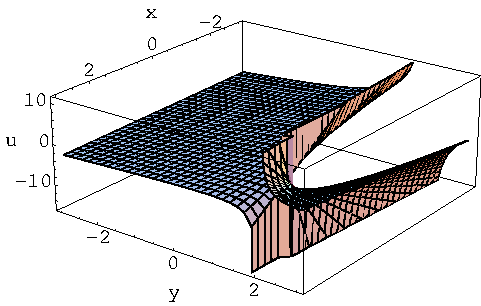
\includegraphics[width=0.5\textwidth]{pde/characteristics/u_sing_y_2}
    \end{center}
    \caption{The solution.}
    \label{u_sing_y_2}
  \end{figure}
\end{Solution}








%%(y + u) u_x + y u_y = x - y, \quad u \big|_{y=1} = 1 + x.
\begin{Solution}
  \begin{equation}
    \label{eqnyuuxyuyxy}
    (y + u) u_x + y u_y = x - y, \quad u \big|_{y=1} = 1 + x
  \end{equation}
  We differentiate $u$ with respect to $s$.
  \[
  \frac{\dd u}{\dd s} = u_x \frac{\dd x}{\dd s} + u_y \frac{\dd y}{\dd s}
  \]
  We compare this with Equation~\ref{eqnyuuxyuyxy} to obtain differential
  equations for $x$, $y$ and $u$.
  \[
  \frac{\dd x}{\dd s} = y + u, \quad
  \frac{\dd y}{\dd s} = y, \quad
  \frac{\dd u}{\dd s} = x - y
  \]
  We parametrize the initial data in terms of $s$.
  \[
  x(s = 0) = \alpha, \quad
  y(s = 0) = 1, \quad
  u(s = 0) = 1 + \alpha
  \]
  We solve the equation for $y$ subject to the inital condition.
  \[
  y(s) = \e^s
  \]
  This gives us a coupled set of differential equations for $x$ and $u$.
  \[
  \frac{\dd x}{\dd s} = \e^s + u, \quad
  \frac{\dd u}{\dd s} = x - \e^s
  \]
  The solutions subject to the initial conditions are
  \[
  x(s) = (\alpha + 1) \e^s - \e^{-s}, \quad
  u(s) = \alpha \e^s + \e^{-s}.
  \]
  We substitute $y(s) = \e^s$ into these solutions.
  \[
  x(s) = (\alpha + 1) y - \frac{1}{y}, \quad
  u(s) = \alpha y + \frac{1}{y}
  \]
  We solve the first equation for $\alpha$ and substitute it into
  the second equation to obtain the solution.
  \[
  u(x,y) = \frac{2 + x y - y^2}{y}
  \]
  This solution is valid for $y > 0$.  The characteristic passing
  through $(\alpha, 1)$ is
  \[
  x(s) = (\alpha + 1) \e^s - \e^{-s}, \quad
  y(s) = \e^s.
  \]
  Hence we see that the characteristics satisfy $y(s) \geq 0$
  for all real $s$.
  Figure~\ref{charm55soln}
  shows some characteristics in the $(x,y)$ plane with starting 
  points from $(-5,1)$ to $(5,1)$ and a plot of the solution.
  \begin{figure}[h!]
    \begin{center}
      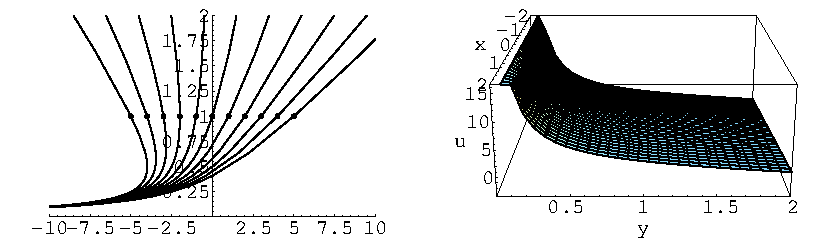
\includegraphics[width=\textwidth]{pde/characteristics/charm55soln}
    \end{center}
    \caption{Some characteristics and the solution.}
    \label{charm55soln}
  \end{figure}
\end{Solution}












\raggedbottom

}
